% ============================================================
%  §6  Discussion: Observation, Recording, and Law
%       — A Reconfiguration via Closure
% ============================================================

\section{Discussion: Observation, Recording, and Law}
\label{sec:discussion}

The question of what constitutes observation remains an open and actively debated problem in
physics.
The present work does not aim to resolve this problem in a definitive sense.
Instead, it introduces a structural perspective in which observation is reinterpreted in terms of
closure dynamics.

Recalling Eq.~\eqref{eq:I-C-relation}, within IFGT information is defined as a
function of closure degree~$C$:
\begin{equation}
  I = f(1 - C).
\end{equation}
As closure increases, differences are progressively resolved, and the capacity for informational
variation diminishes.
In the limit $C \to 1$ we obtain $I \to 0$, corresponding to a state in which no further
distinction can be made.
Such a state, while theoretically defined, does not manifest as an observable phenomenon.

From this viewpoint, observation is not the passive acquisition of a pre-existing state.
Rather, it is an active operation that locally increases closure, projecting an ongoing generative
process into a stable and recordable configuration.
In this sense,
\begin{quote}
  \itshape
  observation may be understood as a local closure operation that projects flow into structure.
\end{quote}

\begin{figure}[h]
  \centering
  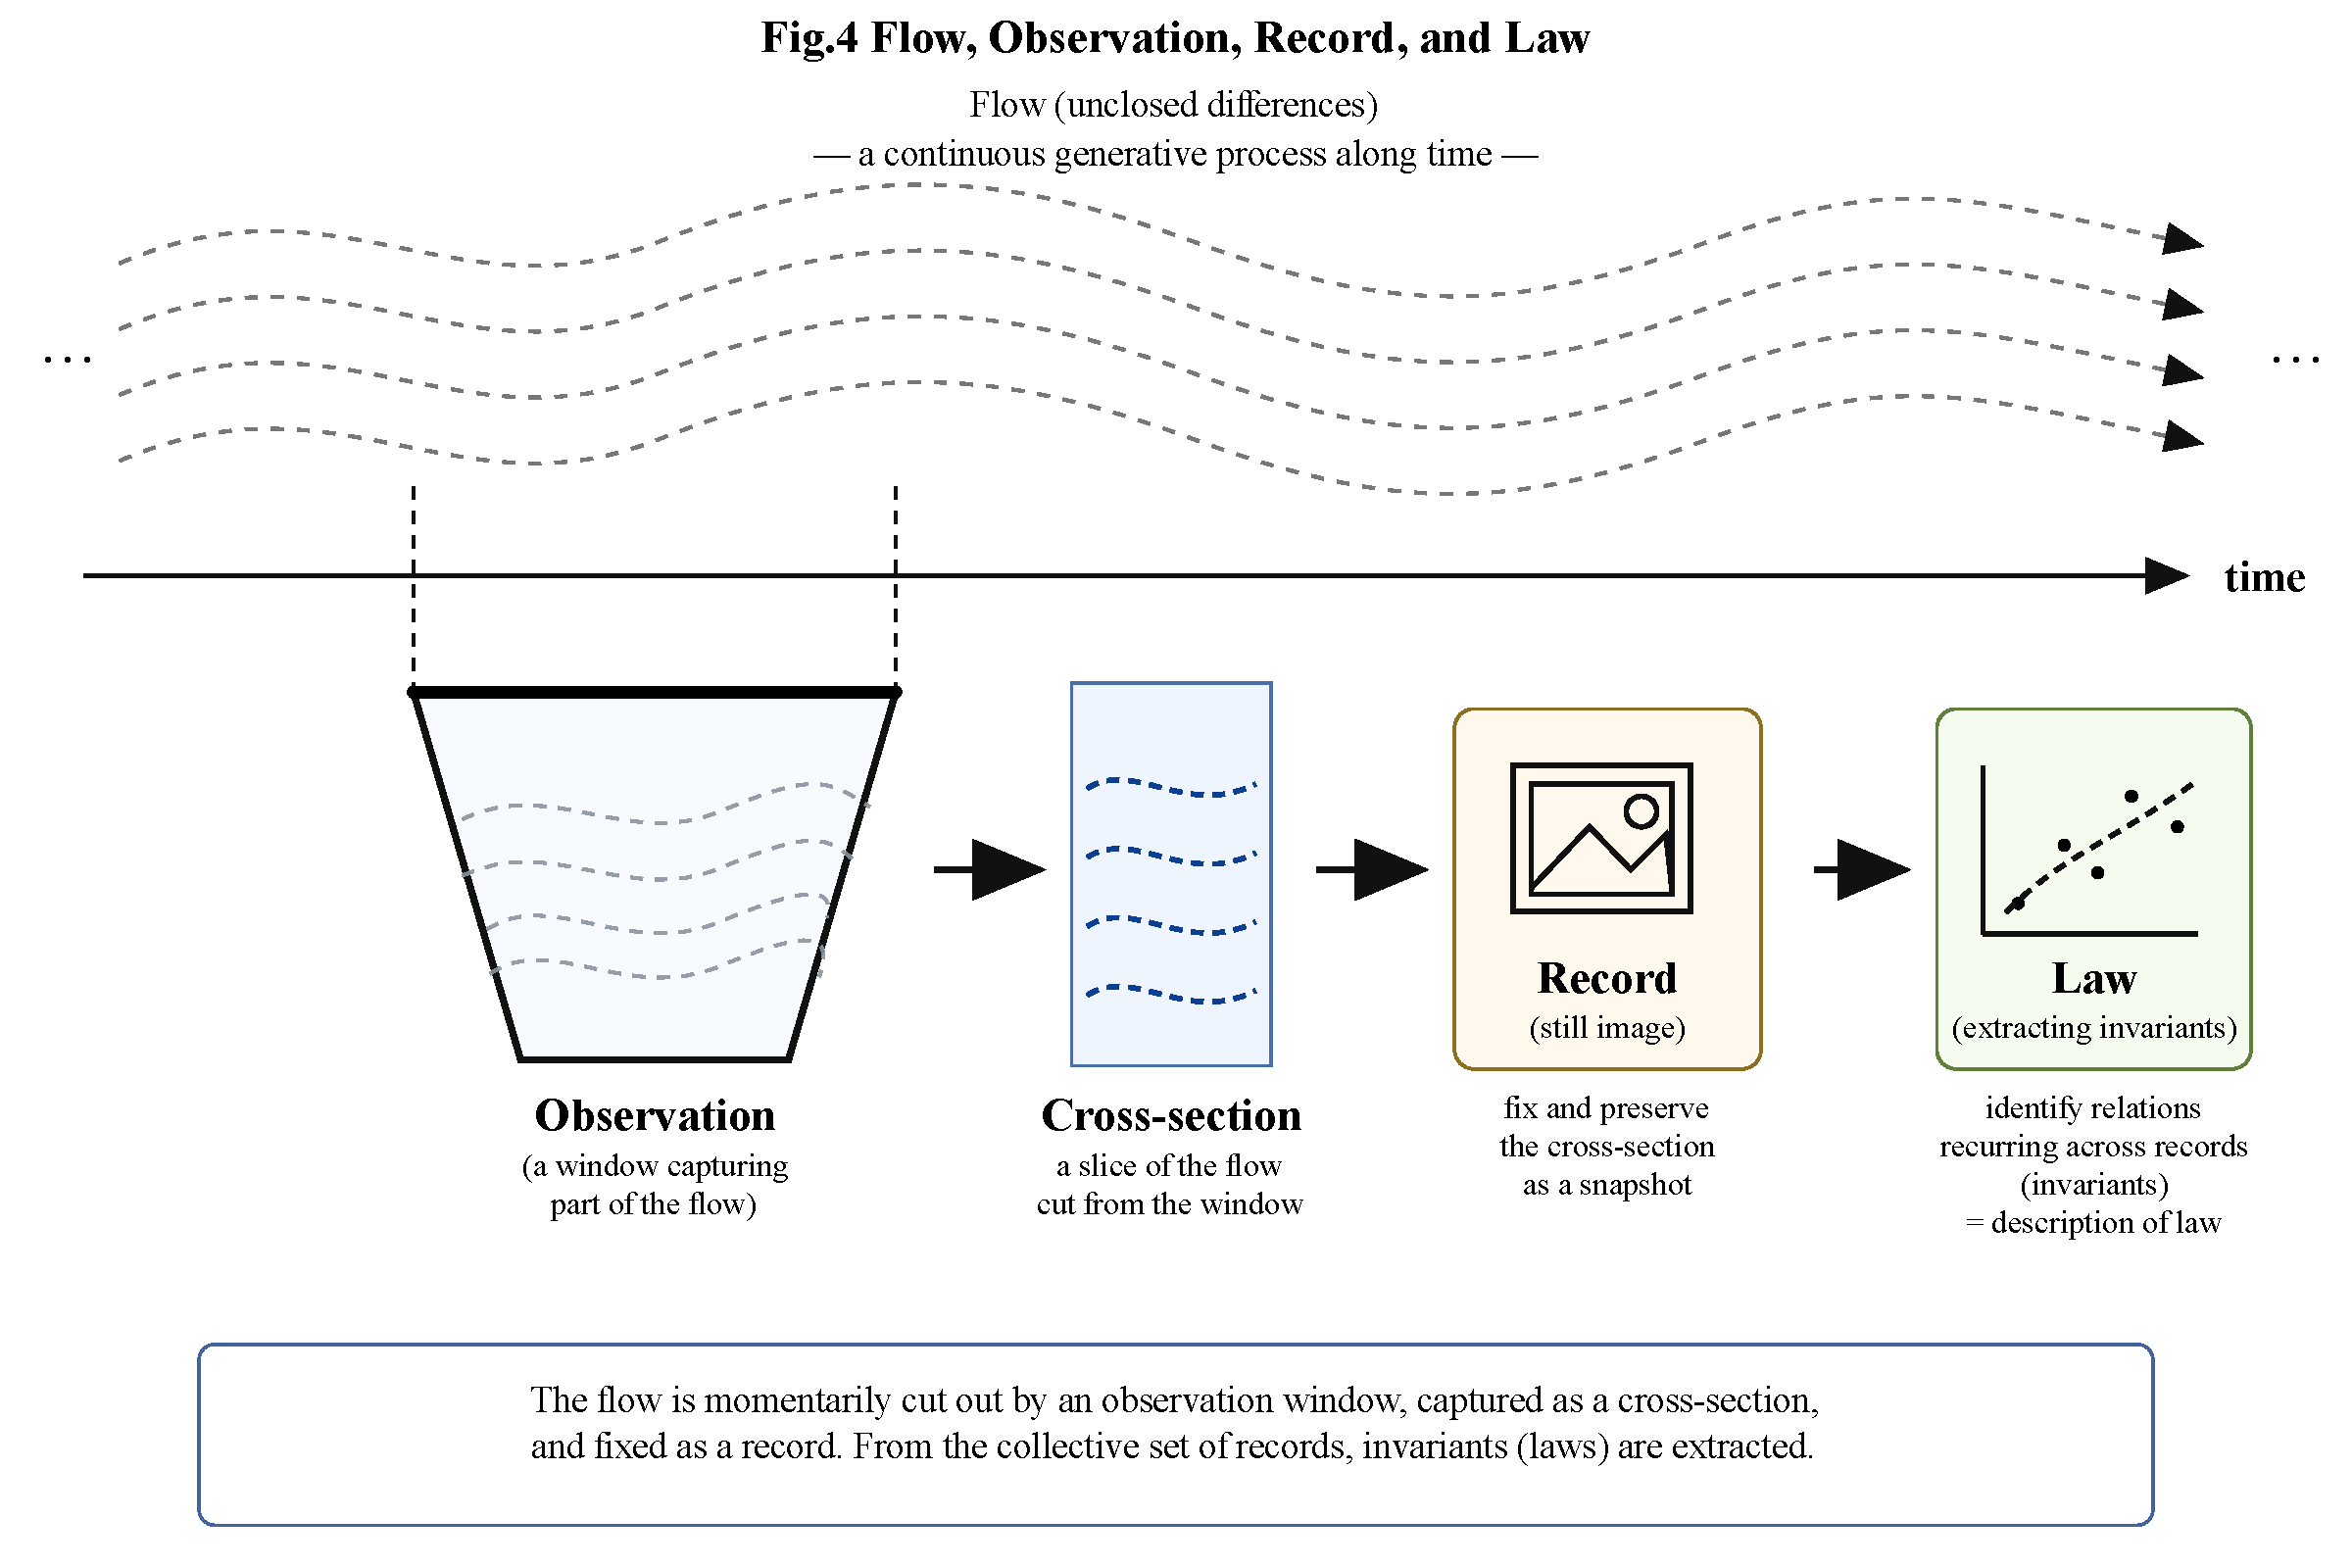
\includegraphics[width=0.88\textwidth]{figures/fig4_observationen_en.pdf}
  \caption{Flow, Observation, Record, and Law.
    The flow is locally cut out by an observation window, captured as a cross-section,
    and fixed as a record.
    From the collective set of records, invariants (laws) are extracted.}
  \label{fig:obs_record_law}
\end{figure}

As a consequence, what is observed appears static.
This apparent stillness is not an intrinsic property of the world itself, but a result of the
observational process.
Even when represented as continuous media such as video or signal streams, observation consists of
a sequence of stabilized cross-sections, rather than direct access to the generative frontier
(see Fig.~\ref{fig:obs_record_law}).

This structure extends naturally to recording.
Recording is not the storage of information as such, but the transformation of differences into
high-closure configurations that can later be reactivated.
Written text, visual imagery, sound, and digital data do not constitute information in themselves;
rather, they function as interference devices that enable the re-emergence of informational
relations.

This perspective also clarifies the status of physical laws.
Laws do not generate the behavior of the world; instead, they are extracted from sequences of
high-closure observational states as stable relations.
That is,
\begin{quote}
  \itshape
  physical laws can be understood as invariants extracted from sequences of high-closure
  cross-sections.
\end{quote}

The apparent stability of the world does not imply simplicity or static structure.
On the contrary, it reflects the existence of a regime in which a large number of invariants
persist across the observational projection of an underlying high-density, high-frequency
dynamical process.
Physical laws are thus traces of dynamical stability, rather than generative principles.

This framework suggests that observable systems should exhibit invariant
structures corresponding to high-closure cross-sections, providing a potential
direction for empirical investigation.

Importantly, this reconfiguration does not invalidate existing physical descriptions.
Atomistic models and law-based formulations remain highly accurate within the domains in which they
operate.
However, they correspond to descriptions in high-closure regimes and do not directly capture the
generative dynamics from which these stable structures emerge.

In the present framework, the starting point is instead placed at a more minimal level:
\begin{quote}
  \itshape
  difference exists.
\end{quote}
From this minimal asymmetry, gradients arise, flows are generated, structures are formed, and
eventually stable invariants appear as observable laws.
In this sense, atoms and laws are not the fundamental drivers of the world, but emergent structures
within an ongoing generative process.

Finally, this perspective offers a natural reinterpretation of classical philosophical problems,
such as Hume's analysis of causation and various thought experiments (e.g., the five-minute
hypothesis or simulation scenarios).
Since observation operates on stabilized configurations, the generative history and origin of a
system are not directly accessible.
These problems thus reflect not a failure of knowledge, but a structural property of observation
itself: it selects high-closure slices of an inherently unclosed process.

Accordingly, the present work does not claim to solve the measurement problem, but rather to
provide an additional structural axis along which it may be reconsidered.
In this context, observation can be understood as an operation that shifts a system toward higher
closure, thereby restricting access to the generative domain that lies toward lower and
intermediate~$C$ (see Eq.~(6) and \S\ref{sec:fundamental_dynamics}).
